\selectlanguage{english}
\chapter{Object reconstruction in CMS}
\label{Chapter1}
\newcommand{\cPqb}{\ensuremath{\cmsSymbolFace{b}}}
%SourceDoc tesi.tex

The global event reconstruction (also called particle-flow event reconstruction~\cite{CMS-PRF-14-001}) aims to reconstruct and identify each individual particle in an event, with an optimized combination of all subdetector information, \figurename~\ref{ParticleFlow}. In this process, the identification of the particle type (photon, electron, muon, charged hadron, neutral hadron) plays an important role in the determination of the particle direction and energy. Photons (\eg  coming from \Pgpz decays or from electron bremsstrahlung) are identified as ECAL energy clusters not linked to the extrapolation of any charged particle trajectory to the ECAL. Electrons %(\eg  coming from photon conversions in the tracker material or from \cPqb-hadron semileptonic decays)%
are identified as a primary charged particle track and potentially many ECAL energy clusters corresponding to this track extrapolation to the ECAL and to possible bremsstrahlung photons emitted along the way through the tracker material. Muons %(\eg  from \cPqb-hadron semileptonic decays)%
are identified as a track in the central tracker consistent with either a track or several hits in the muon system, associated with an energy deficit in the calorimeters. Charged hadrons are identified as charged particle tracks neither identified as electrons, nor as muons. Finally, neutral hadrons are identified as HCAL energy clusters not linked to any charged hadron trajectory, or as ECAL and HCAL energy excesses with respect to the expected charged hadron energy deposit.
%The energy of photons is directly obtained from the ECAL measurement, corrected for zero-suppression effects. The energy of electrons is determined from a combination of the track momentum at the main interaction vertex, the corresponding ECAL cluster energy, and the energy sum of all bremsstrahlung photons attached to the track. The energy of muons is obtained from the corresponding track momentum. The energy of charged hadrons is determined from a combination of the track momentum and the corresponding ECAL and HCAL energy, corrected for zero-suppression effects and for the response function of the calorimeters to hadronic showers. Finally, the energy of neutral hadrons is obtained from the corresponding corrected ECAL and HCAL energy.
%For each event, hadronic jets are clustered from these reconstructed particles using the infrared and collinear safe anti-$k_{t}$ algorithm~\cite{Cacciari:2008gp, Cacciari:2011ma} with a distance parameter of 0.4. The jet momentum is determined as the vectorial sum of all particle momenta in the jet, and is found from simulation to be within 5 to 10\% of the true momentum over the whole $p_{t}$ spectrum and detector acceptance. Additional proton-proton interactions within the same or nearby bunch crossings can contribute additional tracks and calorimetric energy depositions to the jet momentum. To mitigate this effect, tracks identified to be originating from pileup vertices are discarded and an offset correction is applied to correct for remaining contributions. Jet energy corrections are derived from simulation to bring measured response of jets to that of particle level jets on an average. In situ measurements of the momentum balance in dijet, $\text{photon} + \text{jet}$, $\PZ + \text{jet}$, and multijet events are used to account for any residual differences in jet energy scale in data and simulation~\cite{Khachatryan:2016kdb}. The jet energy resolution amounts typically to 15\% at 10 GeV, 8\% at 100 GeV, and 4\% at 1 TeV. Additional selection criteria are applied to each jet to remove jets potentially dominated by anomalous contributions from various subdetector components or reconstruction failures.
\begin{figure}[htbp]
\centering
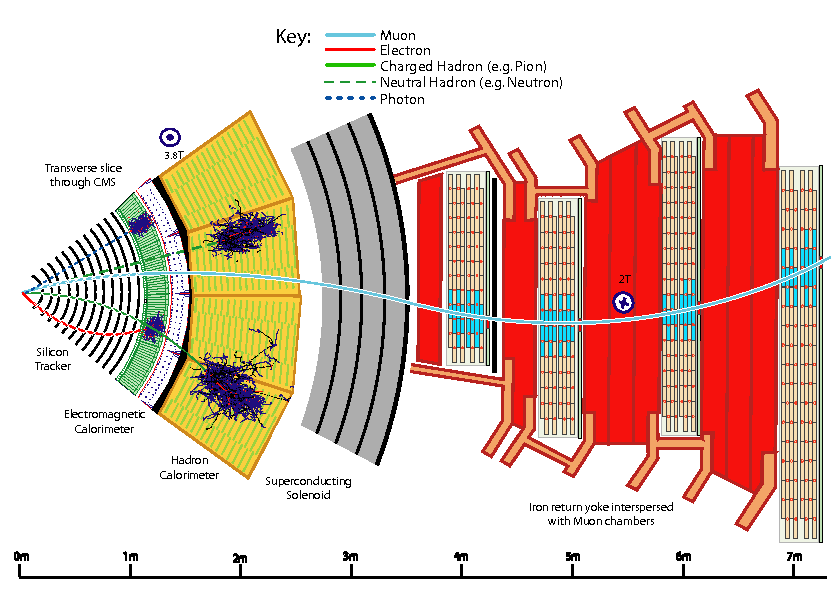
\includegraphics[width=0.7\textwidth]{Images/ParticleFlow}
\caption{Particle interaction and reconstruction in a transverse slice of the CMS detector, from the beam pipe to the muon detector.}
\label{ParticleFlow}
\end{figure}

\section{Photons}
Photons \cite{photons} for use as signals or signatures in measurements and searches, rather than for use in the construction of jets or missing transverse energy, are reconstructed from energy deposits in the ECAL using algorithms that constrain the clusters to the size and shape expected for electrons and photons with \pt  $\ge$15 GeV. The algorithms do not use any hypothesis as to whether the particle originating from the interaction point is a photon or an electron, consequently electrons from $Z \to e^{+}e^{-}$ events, for which pure samples with a well defined invariant mass can be selected, can provide excellent measurements of the photon trigger, reconstruction, and identification efficiencies, and of the photon energy scale and resolution. The reconstructed showers are generally limited to a fiducial region excluding the last two crystals at each end of the barrel ($|\eta | <$ 1.4442). The outer circumferences of the endcaps are obscured by services passing between the barrel and the endcaps, and this area is removed from the fiducial region by excluding the first ring of trigger towers of the endcaps ($|\eta | >$ 1.566). The fiducial region terminates at $|\eta|$ = 2.5 where the tracker coverage ends.The photon reconstruction proceeds through several steps: 
\begin{itemize}
\item calibration: the calorimeter signals in data must be calibrated and corrected for several detector effects
\item clusterisation: clustering algorithms collect the energy from radiating electrons and converted photons that gets spread in the $\phi$ direction by the magnetic field; these algorithms are evolved from fixed matrices of 5 x 5 crystals, which provide the best reconstruction of unconverted photons, by allowing extension of the energy collection in the $\phi$ direction, to form "superclusters"
\item correction of cluster energy: main effects (\eg variation of longitudinal containment, variation of lateral containment or variation in the amount of energy absorbed before reaching the ECAL for showers starting before the ECAL) force to correct the initial sum of energy deposits
\end{itemize}

\section{Electrons}
Electrons \cite{electrons} are reconstructed by associating a track reconstructed in the silicon detector with a cluster of energy in the ECAL. A mixture of a stand-alone approach \cite{electrons_2} and the complementary global particle-flow algorithm is used to maximize the performance. The electron energy usually spreads out over several crystals of the ECAL. This spread can be quite small when electrons lose little energy via bremsstrahlung before reaching ECAL. To measure the initial energy of the electron accurately, it is essential to collect the energy of the radiated photons that mainly spreads along the $\phi$ direction because of the bending of the electron trajectory in the magnetic field. The spread in the $\eta$ direction is usually negligible, except for very low \pt (\pt $<$ 5GeV). Two clustering algorithms, the ?hybrid? algorithm in the barrel, and the "multi-5x5" in the endcaps, are used for this purpose. \\
The starting point of the hybrid algorithm is a seed crystal, defined as the one containing most of the energy deposited in any considered region: arrays of 5 x 1 crystals in $\eta$ x $\phi$ are added around the seed crystal, in a range of $N_{steps}$ crystals in both directions of $\phi$ if their energies exceed a minimum threshold. The contiguous arrays are grouped array into clusters, with each distinct cluster required to have a seed array with energy greater than a threshold in order to be collected in the final global cluster, called the supercluster seed-array (SC). \\
%The multi-5x5 algorithm is used in the ECAL endcaps (EE), where crystals are not arranged in an ? � ? geometry. It starts with the seed crystals, the ones with local maximal energy relative to their four direct n








